\documentclass[12pt]{beamer}
\usepackage{../Estilos/BeamerMAF}
\usepackage{../Estilos/ColoresLatex}
%Sección para el tema de beamer, con el theme, usercolortheme y sección de footers
\usetheme{Frankfurt}
\usecolortheme{beaver}
%\useoutertheme{default}
\setbeamercovered{invisible}
% or whatever (possibly just delete it)
\setbeamertemplate{section in toc}[sections numbered]
\setbeamertemplate{subsection in toc}[subsections numbered]
\setbeamertemplate{subsection in toc}{\leavevmode\leftskip=3.2em\rlap{\hskip-2em\inserttocsectionnumber.\inserttocsubsectionnumber}\inserttocsubsection\par}
% \setbeamercolor{section in toc}{fg=blue}
% \setbeamercolor{subsection in toc}{fg=blue}
% \setbeamercolor{frametitle}{fg=blue}
\setbeamertemplate{caption}[numbered]

\setbeamertemplate{footline}
\beamertemplatenavigationsymbolsempty
\setbeamertemplate{headline}{}


\makeatletter
% \setbeamercolor{section in foot}{bg=gray!30, fg=black!90!orange}
% \setbeamercolor{subsection in foot}{bg=blue!30!yellow, fg=red}
% \setbeamercolor{date in foot}{bg=black, fg=white}
\setbeamertemplate{footline}
{
  \leavevmode%
  \hbox{%
  \begin{beamercolorbox}[wd=.333333\paperwidth,ht=2.25ex,dp=1ex,center]{section in foot}%
    \usebeamerfont{section in foot} \insertsection
  \end{beamercolorbox}%
  \begin{beamercolorbox}[wd=.333333\paperwidth,ht=2.25ex,dp=1ex,center]{subsection in foot}%
    \usebeamerfont{subsection in foot}  \insertsubsection
  \end{beamercolorbox}%
  \begin{beamercolorbox}[wd=.333333\paperwidth,ht=2.25ex,dp=1ex,right]{date in head/foot}%
    \usebeamerfont{date in head/foot} \insertshortdate{} \hspace*{2em}
    \insertframenumber{} / \inserttotalframenumber \hspace*{2ex} 
  \end{beamercolorbox}}%
  \vskip0pt%
}







\setbeamercolor{section in foot}{bg=chartreuse(web), fg=black}
\setbeamercolor{subsection in foot}{bg=naplesyellow, fg=black}
\setbeamercolor{date in foot}{bg=blue, fg=white}

\makeatletter
\setbeamertemplate{footline}
{
\leavevmode%
\hbox{%
\begin{beamercolorbox}[wd=.333333\paperwidth,ht=2.25ex,dp=1ex,center]{section in foot}%
  \usebeamerfont{section in foot} \insertsection
\end{beamercolorbox}%
\begin{beamercolorbox}[wd=.333333\paperwidth,ht=2.25ex,dp=1ex,center]{subsection in foot}%
  \usebeamerfont{subsection in foot}  \insertsubsection
\end{beamercolorbox}%
\begin{beamercolorbox}[wd=.333333\paperwidth,ht=2.25ex,dp=1ex,right]{date in head/foot}%
  \usebeamerfont{date in head/foot} \insertshortdate{} \hspace*{1.5em}
  \insertframenumber{} / \inserttotalframenumber \hspace*{2ex} 
\end{beamercolorbox}}%
\vskip0pt%
}
\makeatother
\usefonttheme{serif}
\setbeamercolor{frametitle}{bg=neoncarrot}
\resetcounteronoverlays{saveenumi}

\date{5 de mayo de 2022}

\title{\large{Polinomios asociados de Legendre}}
\subtitle{Funciones Especiales I}
\author{M. en C. Gustavo Contreras Mayén}

\begin{document}
\maketitle
\fontsize{14}{14}\selectfont
\spanishdecimal{.}

\section*{Contenido}
\frame[allowframebreaks]{\tableofcontents[currentsection, hideallsubsections]}

%Ref. Butkov (1973) 9.8 Spherical Bessel Functions
\section{Polinomios asociados de Legendre}
\frame{\tableofcontents[currentsection, hideothersubsections]}
\subsection{Ecuación  de onda}

\begin{frame}
\frametitle{Uso de los polinomios asociados de Legendre}
La principal utilidad de los polinomios asociados de Legendre es en la expansión de funciones definidas en la superficie de una esfera.
\\
\bigskip
\pause
Veamos el caso con la función de onda.
\end{frame}
\begin{frame}
\frametitle{Función de onda}
Para cada frecuencia fija \pause (Puede ser una eigenfrecuencia determinada a partir de la ecuación radial) \pause $\omega = k \, c$ le corresponde un modo:
\pause
\begin{align*}
\varphi_{k} (\vb{r}, t) = \psi_{k} (\vb{r}) \, \exp(- i \omega t)
\end{align*}
\end{frame}
\begin{frame}
\frametitle{Ecuación de Helmholtz}
Donde $\psi_{k} (\vb{r})$ satisface la ecuación de Helmholtz:
\pause
\begin{align*}
\laplacian{\psi_{k}} + k^{2} \, \psi_{k} = 0
\end{align*}
\end{frame}
\begin{frame}
\frametitle{Resolviendo la ecuación}
Para resolver la ecuación, propongamos una separación de variables del tipo:
\pause
\begin{align*}
\psi_{k} (r, \theta, \phi) = R (r) \, Y (\theta, \phi)
\end{align*}
\pause
que nos lleva a:
\pause
\begin{eqnarray*}
\begin{aligned}
\dv{r} \bigg( r^{2} \, \dv{R}{r} \bigg) &+ \big( k^{2} \, r^{2} + \lambda \big) \, R = 0 \\[0.5em] \pause
\dfrac{1}{\sin \theta} \, \pdv{\theta} \bigg( \sin \theta \, \pdv{Y}{\theta} \bigg) &+ \dfrac{1}{\sin^{2} \theta} \, \pdv[2]{Y}{\phi} + \lambda \, Y = 0
\end{aligned}
\end{eqnarray*}
\end{frame}
\begin{frame}
\frametitle{El tipo de eigenvalor}
El eigenvalor $\lambda$ se determinará a partir de la segunda ecuación, \pause tomemos en cuenta que:
\pause
\setbeamercolor{item projected}{bg=olive,fg=white}
\setbeamertemplate{enumerate items}{%
\usebeamercolor[bg]{item projected}%
\raisebox{1.5pt}{\colorbox{bg}{\color{fg}\footnotesize\insertenumlabel}}%
}
\begin{enumerate}[<+->]
\item $Y (\theta, \phi)$ debe de ser finito para $0 \leq \theta \leq \pi$ y$0 \leq \phi \leq 2 \pi$
\item Tendremos eigenfunciones $Y_{\lambda} (\theta, \phi)$ correspondientes a esos eigenvalores.
\end{enumerate}
\end{frame}
\begin{frame}
\frametitle{Solución completa}
Entonces, la función completa $\phi_{k} (\vb{r})$ se puede expresar por una superposición del tipo:
\pause
\begin{align*}
\psi_{k} (\vb{r}) = \nsum_{\lambda} C_{\lambda} \, R_{\lambda} (r) \, Y_{\lambda} (\theta, \phi)
\end{align*}
\pause
\textbf{Nota: } La suma sobre $\lambda$ debe de considerarse como simbólica, ya que aún no hemos explorado la estructura del espectro de $\lambda$: ya sea continuo o discreto, ya sea que tenga o no degeneración.
\end{frame}
\begin{frame}
\frametitle{Eigenvalores permitidos}
Para establecer los valores permitidos de $\lambda$, completamos la separación de variables, haciendo:
\pause
\begin{align*}
Y (\theta, \phi) = \Theta (\theta) \, \Phi (\phi)
\end{align*}
\end{frame}
\begin{frame}
\frametitle{Nueva separación de variables}
Lo que nos lleva a las ecuaciones:
\pause
\begin{eqnarray*}
\begin{aligned}
\dv{\theta} \bigg( \sin \theta \, \dv{\Theta}{\theta} \bigg) + \bigg( - \sin \theta \lambda + \dfrac{\lambda_{1}}{\sin \theta} \bigg) \, \Theta &= 0 \\[0.5em] \pause
\dv[2]{\Phi}{\phi} - \lambda_{1} \, \Phi &= 0
\end{aligned}
\end{eqnarray*}
las cuales ya hemos resuelto anteriormente.
\end{frame}
\begin{frame}
\frametitle{Propiedad de los eigenvalores}
Sabemos que el espectro de $\lambda_{1}$ es discreto, sea:
\begin{align*}
\lambda_{1} = - m^{2} ~ (m = 0, 1, 2, \ldots)
\end{align*}
\end{frame}
\begin{frame}
\frametitle{Definiendo las eigenfunciones}
Las eigenfunciones pueden definirse de la siguiente manera.
\pause
\\
\noindent
Para $m = 0$:
\pause
\begin{align*}
\Phi_{0} (\phi) = 1
\end{align*}
\pause
para $m \neq 0$:
\begin{align*}
\Phi_{m} (\phi) = \begin{cases}
\cos m \phi & \mbox{o bien} \\
\sin m \phi
\end{cases}
\end{align*}
\end{frame}
\begin{frame}
\frametitle{Ortogonalidad de las funciones}
Estas funciones son ortogonales entre sí y las integrales de normalización son:
\pause
\begin{eqnarray*}
\begin{aligned}
\scaleint{6ex}_{\bs 0}^{2 \pi} \big[ \Phi_{0} (\phi) \big]^{2} \dd{\phi} &= 2 \, \pi \\[0.5em] \pause
\scaleint{6ex}_{\bs 0}^{2 \pi} \cos^{2} m \, \phi \dd{\phi} &= \pi \\[0.5em] \pause
\scaleint{6ex}_{\bs 0}^{2 \pi} \sin^{2} m \, \phi \dd{\phi} &= \pi
\end{aligned}
\end{eqnarray*}
\end{frame}
\begin{frame}
\frametitle{Normalización de las funciones}
Es conveniente en este momento tener esas eigenfunciones \emph{normalizadas a la unidad}, \pause para ello las multiplicamos por las constantes apropiadas para que todas las integrales de normalización sean iguales a la unidad.
\end{frame}
\begin{frame}
\frametitle{Normalización de las funciones}
Esta condición define las funciones normalizadas:
\pause
\begin{eqnarray*}
\begin{aligned}
&\Phi_{0} (\phi) = \dfrac{1}{\sqrt{2 \pi}} \hspace{0.3cm} (m = 0) \\[0.5em] \pause
&\left. \begin{aligned}
\Phi_{m}^{(+)} (\phi) &= \dfrac{1}{\sqrt{\pi}} \, \cos m \, \phi \\[0.5em] \pause
\Phi_{m}^{(-)} (\phi) &= \dfrac{1}{\sqrt{\pi}} \, \sin m \, \phi
\end{aligned} \right\}
(m \neq 0)
\end{aligned}
\end{eqnarray*}
\pause
donde el símbolo $(+)$ o $(-)$ nos recuerda que esas funciones son pares o impares con respecto al intercambio $\phi \leftrightarrow - \phi$.
\end{frame}
\begin{frame}
\frametitle{Espectro de los eigenvalores}
En cuanto a las funciones $\Theta$ se refiere, \pause sabemos que el espectro de $\lambda$ es también discreto, con:
\pause
\begin{align*}
\lambda = - \ell (\ell + 1) \hspace{0.5cm} \ell = 0, 1, 2, \ldots
\end{align*}
pero para cualquier $m$ dado, se tiene que $\ell \geq m$.
\end{frame}
\begin{frame}
\frametitle{Los polinomios asociados de Legendre}
Las soluciones de la ecuación con $\Theta$ son los polinomios asociados de Legendre:
\begin{align*}
P_{\ell}^{m} (\cos \theta)
\end{align*}
\end{frame}
\begin{frame}
\frametitle{Normalización de los $P_{\ell}^{m}$}
Es conveniente normalizarlos a la unidad también, definiendo entonces:
\pause
\begin{align*}
\Theta_{\ell}^{m} (\cos \theta) = \sqrt{\dfrac{2 \ell + 1}{2} \, \dfrac{(\ell - m)!}{(\ell + m)!}} \, P_{\ell}^{m} (\cos \theta)
\end{align*}
\end{frame}
\begin{frame}
\frametitle{Normalizando los $P_{\ell}^{m}$}
Por lo que:
\pause
\begin{eqnarray*}
\begin{aligned}
&\scaleint{6ex}_{\bs 0}^{\pi} \big[ \Theta_{\ell}^{m} (\cos \theta) \big]^{2} \sin \theta \dd{\theta} = \\[0.5em] \pause
&=\dfrac{2 \ell + 1}{2} \, \dfrac{(\ell - m)!}{(\ell + m)!} \, \scaleint{6ex}_{\bs -1}^{+1} \big[ P_{\ell}^{m}  (x) \big]^{2} \dd{x} = \pause 1
\end{aligned}
\end{eqnarray*}
\end{frame}
\begin{frame}
\frametitle{Problema de eigenvalores}
Ahora debería de quedar claro que la ecuación de eigenvalores:
\pause
\begin{align*}
\dfrac{1}{\sin \theta} \, \pdv{\theta} \bigg( \sin \theta \, \pdv{Y}{\theta} \bigg) &+ \dfrac{1}{\sin^{2} \theta} \, \pdv[2]{Y}{\phi} + \lambda \, Y = 0
\end{align*}
\pause
tiene los eigenvalores:
\pause
\begin{align*}
\lambda = - \ell (\ell + 1) \hspace{0.4cm} \ell = 0, 1, 2, \ldots
\end{align*}
\end{frame}
\begin{frame}
\frametitle{Degeneración en las eigenfunciones}
Los eigenvalores son, sin embargo, \pause \emph{degenerados} (excepto si $\ell = 0)$, \pause por que para cada valor fijo de $\ell$, se tiene varias eigenfunciones:
\pause
\begin{eqnarray*}
\begin{aligned}
&\Theta_{\ell}^{0} (\cos \theta) \, \Phi_{0} (\phi) \\[0.5em] \pause
&\Theta_{\ell}^{1} (\cos \theta) \, \Phi_{1}^{(+)} (\phi) \hspace{0.7cm} \Theta_{\ell}^{1} (\cos \theta) \, \Phi_{1}^{(-)} (\phi) \\[0.5em] \pause
&\Theta_{\ell}^{2} (\cos \theta) \, \Phi_{2}^{(+)} (\phi) \hspace{0.7cm} \Theta_{\ell}^{2} (\cos \theta) \, \Phi_{2}^{(-)} (\phi) \\[0.5em] \pause
&{} \hspace{0.3cm} \vdots
\end{aligned}
\end{eqnarray*}
y así sucesivamente.
\end{frame}
\begin{frame}
\frametitle{Eigenfunciones degeneradas}
Hasta llegar a:
\pause
\begin{align*}
\Theta_{\ell}^{\ell} (\cos \theta) \, \Phi_{\ell}^{(+)} (\phi) \hspace{0.5cm} \Theta_{\ell}^{\ell} (\cos \theta) \, \Phi_{\ell}^{(-)} (\phi)
\end{align*}
\pause
Para cada valor de $\ell$ le corresponden $(2 \ell + 1)$ eigenfunciones, teniendo entonces un orden de degeneración de $(2 \ell + 1)$.
\end{frame}
\begin{frame}
\frametitle{Soluciones fundamentales}
Definimos las soluciones fundamentales de la EDP (sujeta a las CDF apropiadas):
\pause
\begin{align*}
\dfrac{1}{\sin \theta} \, \pdv{\theta} \bigg( \sin \theta \, \pdv{Y}{\theta} \bigg) &+ \dfrac{1}{\sin^{2} \theta} \, \pdv[2]{Y}{\phi} + \ell (\ell + 1) \, Y = 0
\end{align*}
\end{frame}
\begin{frame}
\frametitle{Soluciones fundamentales}
Por medio de las expresiones:
\pause
\begin{eqnarray*}
&Y_{\ell 0} (\theta, \phi) = \sqrt{\dfrac{2 \ell + 1}{4 \pi}} \, P_{\ell} (\cos \theta) \hspace{0.3cm} (m = 0)
\end{eqnarray*}
\end{frame}
\begin{frame}
\frametitle{Soluciones fundamentales}
\begin{eqnarray*}
\begin{aligned}
&\left. \begin{aligned}
&Y_{\ell m}^{(+)} (\theta, \phi) = \Theta_{\ell}^{m} (\cos \theta) \, \Phi_{m}^{(+)} (\phi) = \\[0.5em] \pause
&= \sqrt{\dfrac{2 \ell + 1}{2 \pi} \, \dfrac{(\ell - m)!}{(\ell + m)!}} \, P_{\ell}^{m} (\cos \theta) \, \cos m \phi \\[0.5em] \pause
&Y_{\ell m}^{(-)} (\theta, \phi) = \Theta_{\ell}^{m} (\cos \theta) \, \Phi_{m}^{(-)} (\phi) = \\[0.5em] \pause
&= \sqrt{\dfrac{2 \ell + 1}{2 \pi} \, \dfrac{(\ell - m)!}{(\ell + m)!}} \, P_{\ell}^{m} (\cos \theta) \, \sin m \phi
\end{aligned} \right\}
(m \neq 0)
\end{aligned}
\end{eqnarray*}
\end{frame}
\begin{frame}
\frametitle{Nombrando a las soluciones}
Estas soluciones son los armónicos esféricos, en la definición clásica.
\\
\bigskip
\pause
De manera contraria en la definición de los armónicos esféricos en la mecánica cuántica, donde $\cos m \phi$ y $\sin m \phi$ se descartan en favor de $\exp(i m \phi)$ y $\exp(-i m \phi)$.
\end{frame}
\begin{frame}
\frametitle{La solución en series}
Se sigue entonces que la expresión en series para $\psi_{k} (\vb{r})$ es del tipo:
\pause
\begin{align*}
\psi_{k} (\vb{r}) = \nsum_{\lambda} C_{\lambda} \, R_{\lambda} (r) \, Y_{\lambda} (\theta, \phi)
\end{align*}
\end{frame}
\begin{frame}
\frametitle{Solución en series}
Es de la forma:
\pause
\begin{align*}
\psi_{k} (\vb{r}) &= \nsum_{\ell=0}^{\infty} R_{\ell} (r) \bigg[ C_{\ell 0} \, Y_{\ell 0} (\theta, \phi) + \\[0.5em]
&+ \nsum_{m=1}^{\ell} \bigg( C_{\ell m}^{(+)} \, Y_{\ell m}^{(+)} (\theta, \phi) + C_{\ell m}^{(-)} \, Y_{\ell m}^{(-)} (\theta, \phi) \bigg) \bigg]
\end{align*}
\end{frame}
\begin{frame}
\frametitle{Analizando la solución}
Supongamos que $r$ está fijo, \pause entonces $\psi_{k} (\vb{r})$ se convierte en una función solo de $\theta$ y $\phi$, por lo que estaremos tratando con una expresión del tipo:
\pause
\begin{align*}
f (\theta, \phi) &= \nsum_{\ell=0}^{\infty} \bigg[ A_{\ell 0} \, Y_{\ell 0} (\theta, \phi) + \\[0.5em]
&+ \nsum_{m=1}^{\ell} \bigg( A_{\ell m}^{(+)} \, Y_{\ell m}^{(+)} (\theta, \phi) + A_{\ell m}^{(-)} \, Y_{\ell m}^{(-)} (\theta, \phi) \bigg) \bigg]
\end{align*}
\end{frame}
\begin{frame}
\frametitle{Solución válida}
Esta expansión en serie es válida para una función arbitraria $f (\theta, \phi)$, sujeta a las condiciones habituales similares para las series de Fourier, series de Fourier-Legendre, series de Fourier-Bessel, etc.
\end{frame}
\begin{frame}
\frametitle{Reecuperando los coeficientes}
Los coeficientes de la expansión se obtienen multiplicando $f (\theta, \phi)$ por el correspondiente armónico esférico y por el factor $\sin \theta$, para luego integrar sobre los ángulos:
\pause
\begin{eqnarray*}
\begin{aligned}
A_{\ell 0} &= \scaleint{6ex}_{\bs 0}^{\pi} \scaleint{6ex}_{\bs 0}^{2 \pi} f (\theta, \phi) \, Y_{\ell 0} (\theta, \phi) \, \sin \theta \dd{\theta} \dd{\phi} \hspace{0.5cm} (m = 0) \\[0.5em] \pause
A_{\ell m}^{(\pm)} &= \scaleint{6ex}_{\bs 0}^{\pi} \scaleint{6ex}_{\bs 0}^{2 \pi} f (\theta, \phi) \, Y_{\ell 0}^{(\pm)} (\theta, \phi) \, \sin \theta \dd{\theta} \dd{\phi} \hspace{0.5cm} (m \neq 0)
\end{aligned}
\end{eqnarray*}
\end{frame}
\begin{frame}
\frametitle{Observación importante}
El factor $\sin \theta$ que se necesita para la ortogonalidad de las funciones $P_{\ell}^{m}$, tiene la siguiente interpretación geométrica: Un ángulo sólido se define por:
\pause
\begin{align*}
\dd{\Omega} = \dfrac{\dd{S}}{r^{2}}
\end{align*}
donde $\dd{S}$ es el elemento de área de una esfera de radio $r$.
\end{frame}
\begin{frame}
\frametitle{Elemento de área en coord. esféricas}
En el sistema esférico:
\pause
\begin{align*}
\dd{S} = r \, \dd{\theta} \, r \, \sin \theta \dd{\phi}
\end{align*}
\pause
Tal que:
\pause
\begin{align*}
\dd{\Omega} = \sin \theta \dd{\theta} \dd{\phi}
\end{align*}
y las integrales citadas anteriormente pueden considerarse integrales sobre el ángulo sólido.
\end{frame}
\begin{frame}
\frametitle{Integrales sobre el ángulo sólido}
Y escribirse simbólicamente como:
\pause
\begin{eqnarray*}
\begin{aligned}
A_{\ell 0} &= \scaleint{6ex}_{\Omega} f (\Omega) \, Y_{\ell 0} (\Omega) \dd{\Omega} \hspace{0.5cm} (m = 0) \\[0.5em] \pause
A_{\ell m}^{\pm} &= \scaleint{6ex}_{\Omega} f (\Omega) \, Y_{\ell m}^{\pm} (\Omega) \dd{\Omega} \hspace{0.5cm} (m \neq 0)
\end{aligned}
\end{eqnarray*}
\end{frame}

\section{Las funciones esféricas de Bessel}
\frame{\tableofcontents[currentsection, hideothersubsections]}
\subsection{Ec. Onda y de Helmholtz}

\begin{frame}
\frametitle{La ec. de onda}
Continuemos revisando las EDP de onda y de Helmholtz en coordenadas esféricas. \pause Sabemos que la ecuación radial es de la forma:
\pause
\begin{align*}
\dv{r} \bigg( r^{2} \dv{R}{r} \bigg) + \big[ k^{2} r^{2} {-} \ell (\ell {+} 1) \big] R = 0 \hspace{0.5cm} \ell = 0, 1, \ldots
\end{align*}
\end{frame}
\begin{frame}
\frametitle{Haciendo un cambio de variable}
Si hacemos el cambio de variable $x = k \, r$, $y (x) \equiv R (r)$, la ecuación se reduce a:
\pause
\begin{align*}
x^{2} \, \dv[2]{y}{x} + 2 \, x \, \dv{y}{x} + \big[ x^{2} - \ell (\ell + 1) \big] \, y = 0
\end{align*}
\end{frame}
\begin{frame}
\frametitle{soluciones a la ecuación}
Las soluciones de esta ED se conocen como:
\pause
\setbeamercolor{item projected}{bg=olive,fg=white}
\setbeamertemplate{enumerate items}{%
\usebeamercolor[bg]{item projected}%
\raisebox{1.5pt}{\colorbox{bg}{\color{fg}\footnotesize\insertenumlabel}}%
}
\begin{enumerate}[<+->]
\item Las \emph{funciones esféricas de Bessel}: $j_{\ell} (x)$
\item Las funciones \emph{esféricas de Neumann}: $n_{j} (x)$
\end{enumerate}
\pause
de orden $\ell$.
\end{frame}
\begin{frame}
\frametitle{Origen del nombre de las funciones}
La razón de darles ese nombre es debido al cambio de variable:
\pause
\begin{align*}
y (x) = \dfrac{u (x)}{\sqrt{x}}
\end{align*}
\end{frame}
\begin{frame}
\frametitle{Expresión modificada}
Que reduce la ecuación a la forma:
\pause
\begin{align*}
\dv[2]{u}{x} + \dfrac{1}{x} \dv{u}{x} + \bigg[ 1 - \dfrac{\big( \ell + \frac{1}{2} \big)}{x^{2}} \bigg] \, u = 0 \hspace{0.5cm} \ell = 0, 1, 2, \ldots
\end{align*}
\pause
que reconocemos es la ED de Bessel de orden $\ell + 1/2$.
\end{frame}
\begin{frame}
\frametitle{Soluciones de la ED}
Se sigue entonces que las soluciones de la ED inicial, pueden escribirse de la forma:
\pause
\begin{align*}
y (x) = C_{1} \, \dfrac{J_{\ell+1/2} (x)}{\sqrt{x}} + C_{2} \, \dfrac{J_{-\ell-1/2} (x)}{\sqrt{x}}
\end{align*}
\end{frame}
\begin{frame}
\frametitle{Solución finita en el origen}
Si la función de Bessel esférica $j_{\ell} (x)$ se define como una solución finita en $x = 0$, \pause se sigue que debe ser un múltiplo de $J_{\ell+1/2} (x) / \sqrt{x}$.
\\
\bigskip
\pause
El factor de proporcionalidad generalmente se elige para que sea $\sqrt{\pi/2}$, por lo tanto:
\pause
\begin{align*}
j_{\ell} (x) = \sqrt{\dfrac{\pi}{2 x}} \, J_{\ell+1/2} (x)
\end{align*}
\end{frame}
\begin{frame}
\frametitle{Relación entre funciones}
La relación de las $j_{\ell} (x)$ con las funciones de Bessel, nos permiten expresar las $j_{\ell} (x)$ en términos de $j_{0} (x)$. \pause De la expresión:
\pause
\begin{align*}
J_{\mu+1} (x) = - x^{\mu} \, \dv{x} \bigg[ \dfrac{J_{\mu} (x)}{x^{\mu}} \bigg]
\end{align*}
\end{frame}
\begin{frame}
\frametitle{Nuevo cambio de variable}
Que entonces, al hacer $\mu = \ell + 1/2$ y dividiendo entre $x^{\ell+3/2}$, se tiene:
\pause
\begin{eqnarray*}
\begin{aligned}
\dfrac{J_{\ell+3/2} (x)}{x^{\ell+3/2}} &= - \dfrac{1}{x} \, \dv{x} \bigg[ \dfrac{J_{\ell+1/2} (x)}{x^{\ell+1/2}} \bigg] \\[0.5em] \pause
\mbox{o } \hspace{0.3cm} \dfrac{j_{\ell+1} (x)}{x^{\ell+1}} &= - \dfrac{1}{x} \dv{x} \bigg[ \dfrac{j_{\ell} (x)}{x^{\ell}} \bigg]
\end{aligned}
\end{eqnarray*}
\end{frame}
\begin{frame}
\frametitle{Valores con $\ell$}
Comenzando con $\ell = 0$ y ocupando esta expresión $\ell$ veces, se obtiene:
\pause
\begin{align*}
j_{\ell} (x) = x^{\ell} \bigg( - \dfrac{1}{x} \, \dv{x} \bigg)^{\ell} \, j_{0} (x) \hspace{0.5cm} \ell = 1, 2, \ldots 
\end{align*}
\end{frame}
\begin{frame}
\frametitle{Expresión para valores de $j_{0}$}
Esta expresión únicamente define todas las $j$ funciones una vez que $j_{0}$ se elige. Nuestra ecuación para $\ell = 0$ es entonces:
\pause
\begin{align*}
\dv[2]{y}{x} + \dfrac{2}{x} \, \dv{y}{x} + y = 0
\end{align*}
\end{frame}
\begin{frame}
\frametitle{Resolviendo la ED}
Resolviendo esta ecuación (ya sea por Frobenius o por otro método), \pause encontramos que las funciones $\sin x /x$ y $\cos x /x$ están entre las soluciones.
\\
\bigskip
\pause
Es común definir:
\pause
\begin{align*}
j_{0} (x) = \dfrac{\sin x}{x}
\end{align*}
\end{frame}
\begin{frame}
\frametitle{Comparando el resultado}
En comparación con $J_{1/2}$, se tiene:
\pause
\begin{align*}
j_{0} (x) = \sqrt{\dfrac{\pi}{2 x}} \, J_{1/2} (x)
\end{align*}
que explica el factor $\sqrt{\pi / 2}$.
\end{frame}
\begin{frame}
\frametitle{Segunda  solución}
Las funciones esféricas de Neumann $n_{\ell} (x)$ se generan de manera similar a partir de $n_{0} (x)$ por medio de:
\pause
\begin{align*}
n_{\ell} (x) = x^{\ell} \bigg( - \dfrac{1}{x} \, \dv{x} \bigg)^{\ell} \, n_{0} (x) \hspace{0.5cm} \ell = 1, 2, \ldots
\end{align*}
\end{frame}
\begin{frame}
\frametitle{Definición de $n_{0}$}
Siendo común definir:
\pause
\begin{align*}
n_{0} (x) = - \dfrac{\cos x}{x} = \sqrt{\dfrac{\pi}{2 x}} \, J_{-1/2} (x)
\end{align*}
\end{frame}
\begin{frame}
\frametitle{Algunas funciones $j_{\ell} (x)$}
A continuación se presenta una lista con algunas funciones $j_{\ell} (x)$:
\pause
\begin{eqnarray*}
\begin{aligned}
j_{0} (x) &= \dfrac{\sin x}{x} \\[0.5em] \pause
j_{1} (x) &= \dfrac{\sin x}{x^{2}} - \dfrac{\cos x}{x} \\[0.5em] \pause
j_{2} (x) &= \bigg( \dfrac{3}{x^{3}} - \dfrac{1}{x} \bigg) \, \sin x - \dfrac{3}{x^{2}} \, \cos x \\[0.5em] \pause
j_{3} (x) &= \bigg( \dfrac{15}{x^{4}} - \dfrac{6}{x^{2}} \bigg) \, \sin x - \bigg( \dfrac{15}{x^{3}} - \dfrac{1}{x} \bigg) \, \cos x 
\end{aligned}
\end{eqnarray*}
\end{frame}
\begin{frame}
\frametitle{Gráfica de las $j_{\ell} (x)$}
\begin{figure}[H]
    \centering
    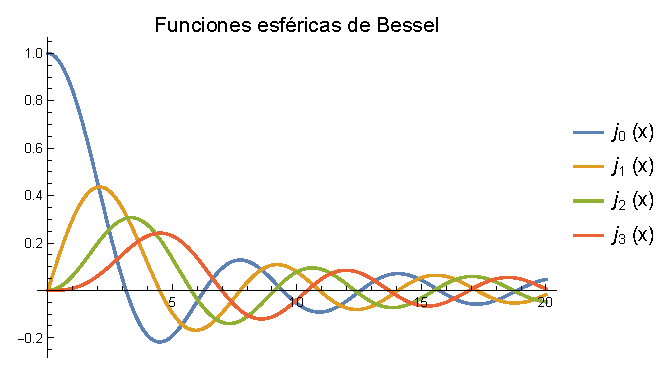
\includegraphics[scale=1]{Imagenes/Plot_Esfericas_Bessel.eps}
\end{figure}
\end{frame}
\begin{frame}
\frametitle{Algunas funciones $n_{\ell} (x)$}
En la siguiente lista ahora presentamos algunas funciones $n_{\ell} (x)$:
\pause
\begin{eqnarray*}
\begin{aligned}
n_{0} (x) &= - \dfrac{\cos x}{x} \\[0.5em] \pause 
n_{1} (x) &= - \dfrac{\cos x}{x^{2}} - \dfrac{\sin x}{x} \\[0.5em] \pause 
n_{2} (x) &= - \bigg( \dfrac{3}{x^{2}} - \dfrac{1}{x} \bigg) \, \cos x - \dfrac{3}{x^{2}} \, \sin x \\[0.5em] \pause 
n_{3} (x) &= - \bigg( \dfrac{15}{x^{4}} - \dfrac{6}{x^{2}} \bigg) \, \cos x - \bigg( \dfrac{15}{x^{3}} - \dfrac{1}{x} \bigg) \, \sin x
\end{aligned}
\end{eqnarray*}
\end{frame}
\begin{frame}
\frametitle{Observación importante}
Las funciones esféricas de Bessel están relacionadas con las funciones de Neumann, por la expresión:
\pause
\begin{align*}
n_{\ell} = \sqrt{\dfrac{\pi}{2 x}} \, N_{l+1/2} (x)
\end{align*}
Es un buen ejercicio demostrar que $N_{\ell+1/2} (x)$ es proporcional a $J_{-\ell-1/2} (x)$, \pause sin embargo, esto es cierto solo si $\ell$ es un número entero.
\end{frame}
\begin{frame}
\frametitle{Gráfica de las $n_{\ell} (x)$}
\begin{figure}[H]
    \centering
    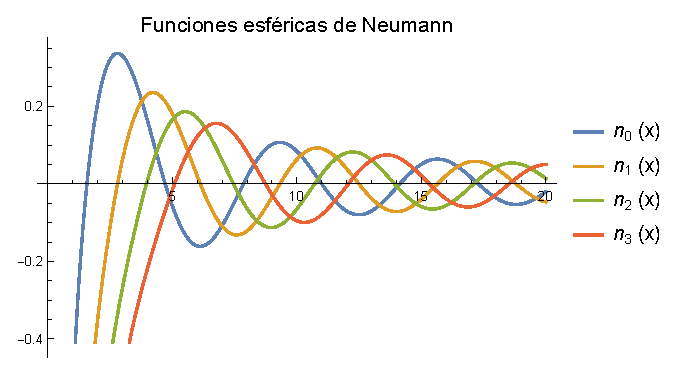
\includegraphics[scale=0.95]{Imagenes/Plot_Esfericas_Neumann.eps}
\end{figure}
\end{frame}

\section{Ejercicio}
\frame{\tableofcontents[currentsection, hideothersubsections]}
\subsection{Ondas estacionarias}

\begin{frame}
\frametitle{Enunciado del ejercicio}
Dentro de una cavidad esférica de radio $a$ se generan ondas sonoras.
\\
\bigskip
\pause
Se desea investigar los patrones de ondas estacionarias dentro de la cavidad y sus frecuencias.
\end{frame}
\begin{frame}
\frametitle{Comenzando la solución}
El problema se puede formular en términos del potencial de velocidad que debe satisfacer la ecuación de onda:
\pause
\begin{align*}
\laplacian{\varphi} - \dfrac{1}{c^{2}} \, \pdv[2]{\varphi}{t} = 0
\end{align*}
\pause
Se supone que la fuente del sonido se elimina en $t = 0$ y se deja que el aire en la cavidad vibre libremente.
\end{frame}
\begin{frame}
\frametitle{Condiciones de frontera}
El problema está sujeto a la CDF:
\pause
\begin{align*}
\pdv{\varphi}{r} \eval_{r = a} = 0
\end{align*}
\end{frame}
\begin{frame}
\frametitle{Tipo de soluciones}
Estamos buscando soluciones de la forma:
\pause
\begin{align*}
\varphi_{k} (\vb{r},  t) = \psi_{k} (\vb{r}) \, \exp(-i \omega t) \hspace{0.7cm} (\omega = k \, c)
\end{align*}
\pause
tal que $\psi_{k} (\vb{r},  t)$ deba satisfacer:
\pause
\begin{align*}
\laplacian{\psi}_{k} + k^{2} \, \psi_{k} = 0 \hspace{0.4cm} \mbox{y} \hspace{0.4cm} \pdv{\psi_{k}}{r} \eval_{r = a} = 0 
\end{align*}
\end{frame}
\begin{frame}
\frametitle{Uso de los resultados anteriores}
De los resultados obtenidos previamente en este material, se tiene que:
\pause
\begin{align*}
&\psi_{k} (\vb{r}) = \nsum_{\ell=0}^{\infty} R_{\ell} (r) \bigg[ C_{\ell 0} \, Y_{\ell 0} (\theta, \phi) + \\[0.5em]
&+ \nsum_{m=0}^{\ell} \bigg( C_{\ell m}^{(+)} \, Y_{\ell m}^{(+)} (\theta, \phi) + C_{\ell m}^{(-)} \, Y_{\ell m}^{(-)} (\theta, \phi) \bigg) \bigg]
\end{align*}
donde los $Y_{\ell m}$ son los armónicos esféricos.
\end{frame}
\begin{frame}
\frametitle{La ecuación radial}
Las funciones $R (r)$ deben de cumplir con la EDO:
\pause
\begin{align*}
\dv{r} \bigg( r^{2} \dv{R_{\ell}}{r} \bigg) &+ \big[ k^{2} r^{2} {-} \ell (\ell + 1) \big] R_{\ell} = 0 \\[0.5em]
&\ell = 0, 1, 2, \ldots
\end{align*}
\end{frame}
\begin{frame}
\frametitle{Solución general a la ec. radial}
La solución general de esta ecuación es del tipo:
\pause
\begin{align*}
R_{\ell} (r) = A_{\ell} \, j_{\ell} (k r) + B_{\ell} \, n_{\ell} (k r) 
\end{align*}
\end{frame}
\begin{frame}
\frametitle{Congruencia con la física}
Ya que la función $n_{\ell} (k r)$ no es finita en $r = 0$, \pause debe de descartarse haciendo que $B_{\ell} = 0$.
\\
\bigskip
\pause
Los valores permitidos de $k$ están determinados por la CDF, lo que se reduce a:
\begin{align*}
\dv{r} j_{\ell} (k r) \eval_{r=a} = 0
\end{align*}
\end{frame}
\begin{frame}
\frametitle{Raíces de la función especial}
Las raíces de $\dv*{x} j_{\ell} (x)$ se pueden encontrar en tablas o mediante el uso de software matemático.
\pause
\begin{table}[H]
\centering
\large
\renewcommand{\arraystretch}{0.9}
\begin{tabular}{c c c}
$\ell$ & $n$ & $\alpha_{\ell n}$ \\ \hline
$0$ & $1$ & $0.0000$ \\ \hline
$1$ & $1$ & $0.6626$ \\ \hline
$2$ & $1$ & $1.0638$ \\ \hline
$0$ & $2$ & $1.4303$ \\ \hline
$3$ & $1$ & $1.4369$ \\ \hline
\end{tabular}
\end{table}
\end{frame}
\begin{frame}
\frametitle{Valores de $k$}
Los correspondientes valores de $k$ para nuestro problema, son los dados por:
\pause
\begin{align*}
k_{\ell n} = \dfrac{\pi \alpha_{\ell n}}{a}
\end{align*}
\pause
y las correspondientes frecuencias están dadas de modo que:
\begin{align*}
\omega_{\ell n} = \dfrac{c \pi \alpha_{\ell n}}{a}
\end{align*}
\end{frame}
\begin{frame}
\frametitle{Estudiando los resutados}
El modo con la frecuencia más baja es para $\ell = 1$ y $n = 1$.
\\
\bigskip
\pause
El caso $\ell = 0$ y $n = 1$, lleva a $\varphi (\vb{r}, t) = \mbox{ constante}$ que puede mantenerse en la solución, pero no corresponde a ninguna onda de sonido congruente con la física (considera que $\vb{v} = - \grad{\varphi})$.
\end{frame}
\begin{frame}
\frametitle{El caso con $\ell = 1$ y $n = 1$}
Las distribuciones angulares son:
\pause
\begin{eqnarray*}
\begin{aligned}
Y_{10} &= \sqrt{\dfrac{3}{4 \pi}} \, \cos \theta \\[0.5em] \pause
Y_{11}^{(+)} &= \sqrt{\dfrac{3}{8 \pi}} \, \sin \theta \cos \phi \\[0.5em] \pause
Y_{11}^{(-)} &= \sqrt{\dfrac{3}{8 \pi}} \, \sin \theta \sin \phi
\end{aligned}
\end{eqnarray*}
\pause
y la función radial es: $j_{1} (k_{11} r)$.
\end{frame}
\begin{frame}
\frametitle{Siguiente modo con $\ell = 2, n= 1$}
El siguiente modo es para $\ell = 2, n= 1$, que tiene un orden de degeneración de $5$:
\pause
\begin{align*}
Y_{20}, \hspace{0.2cm} Y_{21}^{(+)}, \hspace{0.2cm} Y_{21}^{(-)}, \hspace{0.2cm} Y_{22}^{(+)}, \hspace{0.2cm} Y_{22}^{(-)}
\end{align*}
\pause
la función radial es: $j_{2} (k_{21} r)$.
\end{frame}
\begin{frame}
\frametitle{Caso no degenerado}
Se tiene un modo no degenerado con $\ell = 0, n = 2$ y con $j_{0} (k_{02} r)$ y así sucesivamente.
\end{frame}
\begin{frame}
\frametitle{Solución general}
La solución global del problema está dada por la expansión:
pause
\begin{align*}
\varphi (\vb{r}, t) &= \nsum_{n} \nsum_{\ell} \nsum_{m} j_{\ell} (k r) \, Y_{\ell m} (\theta, \phi) \times \\[0.5em]
&\times \bigg[ C_{n \ell m} \exp(-i \omega t) + C_{n \ell m}^{*} \exp(i \omega t) \bigg]
\end{align*}
\end{frame}
\begin{frame}
\frametitle{De los coeficientes}
Los coeficientes $C_{n \ell m}$, en realidad $C_{n \ell 0}, C_{n \ell m}^{(+)}, C_{n \ell m}^{(-)}$, \pause pueden determinarse de las condiciones iniciales las cuales deberían de especificar la distribución inicial del potencial de velocidad $\varphi (\vb{r}, 0)$ \pause y de su derivada temporal $\pdv*{\varphi}{t} (\vb{r}, 0)$, que es proporcional a un cambio fracciona en la densidad.
\end{frame}
\end{document}